\section{Case Study: eBPF}

In this section, we apply the \emph{Code-survey} methodology to analyze the evolution and development of the eBPF subsystem in the Linux kernel. We aim to uncover deep insights into the life cycle, stability, and design decisions of key eBPF features. The results generated by the survey are validated through expert review, as well as quantitative and qualitative analysis.

The Extended Berkeley Packet Filter (eBPF)\cite{ebpf} is a rapidly evolving subsystem in the Linux kernel that allows users to run sandboxed programs in kernel space without modifying the kernel itself \cite{lim2024safebpf}. Originally developed for packet filtering, eBPF now supports diverse use cases like performance tracing, security monitoring, and system observability, and also expand to multiple platforms\cite{windows-ebpf, zheng2023bpftime}. The academic also identifies the current problem and limitation of eBPF, and proposes several works to improve the verifier, deployment.


\subsection{Motivation: Features in eBPF Kernel with Data Analysis}

Let's see how traditional data analysis can bring. With traditional methods and well-defined kernel commits, we can analyze the eBPF kernel feature datasets to study the evolution of various eBPF features, such as helpers, maps, attach types, and other functionalities. We obtained the feature pairs from eBPF-docs\cite{ebpfdocs}, and combined them with Git commit data.

\subsubsection{How Do All eBPF Features Evolve Over Time?}

\Cref{fig:cumulative_feature_timeline} shows trends in the adoption of new features on the overall eBPF subsystem.

\begin{figure}[ht]
    \centering
    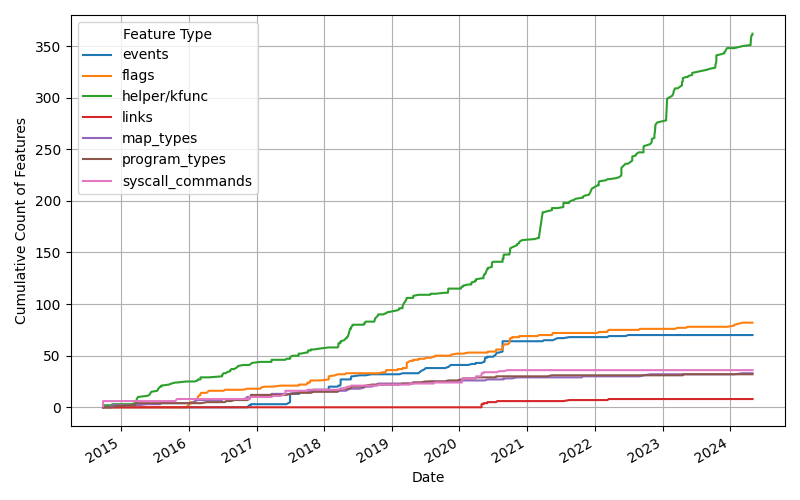
\includegraphics[width=\linewidth]{feature-analysis/cumulative_bpf_features_timeline.png}
    \caption{Cumulative eBPF Features Timeline}
    \label{fig:cumulative_feature_timeline}
\end{figure}

\paragraph{Key Takeaways:}

\begin{enumerate}
    \item \textbf{Helpers and kfuncs} show the most growth for different use cases and changes.
    \item \textbf{Other features} see steady increases in the past 4 years, indicating their maturity.
\end{enumerate}

\subsubsection{Timeline of eBPF Helper Functions vs.\ Kernel Functions}

\Cref{fig:cumulative_helper_kfunc_timeline} shows the evolution of eBPF helper functions and kfuncs over time. 

\begin{figure}[ht]
    \centering
    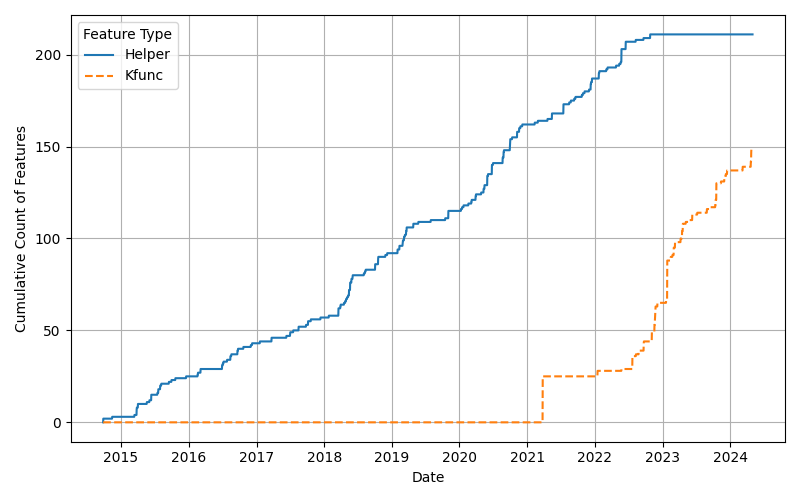
\includegraphics[width=\linewidth]{feature-analysis/cumulative_helper_kfunc_timeline.png}
    \caption{Cumulative Helper and kfunc Timeline}
    \label{fig:cumulative_helper_kfunc_timeline}
\end{figure}

\paragraph{Key Takeaways:}

\begin{enumerate}
    \item \textbf{Helper functions} have been stable since 2023, and almost no new helpers are being added.
    \item \textbf{kfuncs} are growing very rapidly, showing the community's interest in expanding kernel interaction via kfuncs.
    \item All new use cases now tend to use \textbf{kfuncs} to influence kernel behavior, signaling a shift towards deeper kernel integrations.
\end{enumerate}

\subsubsection{What Are the Patterns in Other eBPF Features?}

\Cref{fig:cumulative_without_helper_timeline} examines eBPF feature evolution, excluding helpers and kfuncs. The focus is on core eBPF features and their impact on the overall subsystem.

\begin{figure}[ht]
    \centering
    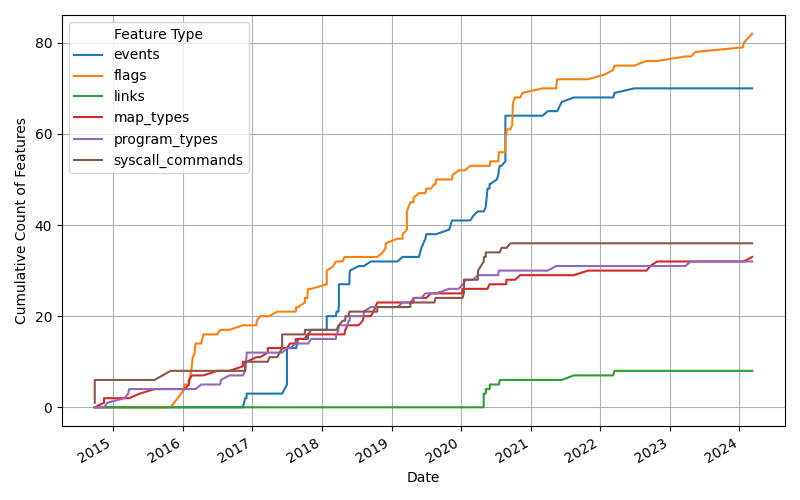
\includegraphics[width=\linewidth]{feature-analysis/cumulative_bpf_features_timeline_no_helper_kfunc.png}
    \caption{Cumulative eBPF Features Timeline Without Helpers and kfuncs}
    \label{fig:cumulative_without_helper_timeline}
\end{figure}

\paragraph{Key Takeaways:}

\begin{enumerate}
    \item \textbf{Core features} like events, flags, map types, and program types have stabilized after 2020.
    \item The introduction of \texttt{bpf\_link} greatly helps manage growing use cases and complexity, shows a significant difference before and after introduced.
\end{enumerate}

\paragraph{However\ldots}

The analysis of eBPF features mainly relies on kernel structured definitions and data sources obtained by humans, which is limited by the availability of data, and the time-consuming process of manual data collection.

There are massive amounts of unstructured data in the form of commit messages, code changes, and developer discussions that can provide valuable insights into the evolution and design decisions of eBPF features. While it is possible for humans to perform empirical analysis on some of this data, covering all of it is practically \emph{impossible}.

\textbf{Can AI assist us?} Instead of letting large language models (LLMs) attempt kernel coding, relying on retrieval-augmented generation (RAG) and fine-tuning to answer questions or code-review—which may yield incorrect answers—we propose a different quantitative approach.

By carefully designing a \emph{survey} and utilizing LLMs to \emph{transform} unstructured data like commits and emails into well-organized, structured, and easy-to-analyze datasets, we can perform \textbf{quantitative} analysis using traditional methods. In this way, AI can help analyze data and provide answers quickly; this capability is already a feature of platforms like ChatGPT.

\subsection{Research Questions for Survey Evaluation}

How can we ensure LLM is not answer questions randomly? To evaluate the effectiveness and correctness of the \emph{Code-survey} results, we explore the following high-level research questions:

\begin{itemize}
    \item \textbf{Correctness of Survey Responses:} How can we ensure that survey responses reflect accurate and relevant information about the system's features and commits?
    \item \textbf{Consistency Across Similar Questions:} Are similar questions answered consistently across different but related features or subsystems?
    \item \textbf{Coverage of Survey Questions:} Do the survey questions comprehensively cover all relevant aspects of the feature or subsystem under analysis?
    \item \textbf{Insight from Survey:} Can the survey data help user analysis the design, implementation, maintenance, reliability and security evlovment and gain valuable insights?
    \item \textbf{Clarity and Ambiguity in Responses:} Are the survey responses clear and unambiguous, making them actionable for further analysis?
    \item \textbf{Alignment with Real-World Changes:} How accurately do survey results reflect real-world changes in the software’s features and evolution?
    \item \textbf{Expert Confirmation:} How do experts rate the accuracy of the survey's generated insights?
\end{itemize}

\subsection{Commit Survey Design and Objectives}

To gain deeper insights into the design and evolution of the eBPF subsystem, we first developed a comprehensive survey aimed at classifying commits within the Linux eBPF subsystem. This survey evaluates specific aspects of each commit by analyzing commit messages and associated code changes. In cases where the commit message provides insufficient information, respondents are allowed to select an "I'm not sure" option.

The primary goals of the survey are to:

\begin{itemize} \item Provide concise summaries of each commit. \item Extract key themes and components affected by each commit. \item Classify commits based on their type, complexity, and impacted components. \item Identify patterns and trends in the evolution of the eBPF subsystem. \end{itemize}

\subsubsection{Survey Structure}

The survey consists of a series of structured questions designed to capture the essential characteristics of each commit. Respondents are encouraged to be as specific as possible based on the available commit message and code changes. If the commit message lacks clarity, the "I'm not sure" option can be selected.

\subsubsection{Simplified Survey Definition}

Below is the simplified survey structure:

\begin{enumerate}
    \item \textbf{Summary}: Provide a one-sentence summary of the commit (max 30 words).
    \item \textbf{Keywords}): Extract up to three keywords from the commit.
    \item \textbf{Commit Classification} (\emph{Single Choice}): What is the main type of the commit?
    \begin{enumerate}[label=(\alph*)]
        \item Bug fix
        \item New feature
        \item Performance optimization
        \item Code cleanup or refactoring
        \item Documentation change or typo fix
        \item Test case or test infrastructure change
        \item Build system or CI/CD change
        \item Security fix
        \item Merge commit
        \item Other type of commit
        \item I'm not sure
    \end{enumerate}
    \item \textbf{Commit Complexity} (\emph{Single Choice}): Estimate the complexity of implementing this commit.
    \begin{enumerate}[label=(\alph*)]
        \item Simple (affects 1--20 lines or 1--2 files)
        \item Moderate (affects 21--100 lines or a few files)
        \item Complex (affects over 100 lines or 5+ files)
        \item Merge-like (merges multiple branches or features)
        \item Non-code or generated changes
        \item I'm not sure
    \end{enumerate}
    \item \textbf{Major Related Implementation Component} (\emph{Single Choice}): What is the main implementation component modified?
    \begin{enumerate}[label=(\alph*)]
        \item eBPF verifier
        \item eBPF JIT compiler
        \item Helpers and kfuncs
        \item Syscall interface
        \item eBPF maps
        \item \texttt{libbpf} library
        \item \texttt{bpftool} utility
        \item Test cases and makefiles
        \item Changes in other subsystems related to eBPF events
        \item Merge commit
        \item Other component related to eBPF
        \item Unrelated to eBPF subsystem
        \item I'm not sure
    \end{enumerate}
    \item \textbf{Major Related Logic Component} (\emph{Single Choice}): What is the main logic component affected?
    \begin{enumerate}[label=(\alph*)]
        \item eBPF instruction logic
        \item Runtime features logic
        \item eBPF events-related logic
        \item Control plane interface logic
        \item Maps logic
        \item BPF Type Format (BTF) logic
        \item Merge commit
        \item General utilities logic
        \item Other eBPF logic component
        \item Unrelated to eBPF subsystem
        \item I'm not sure
    \end{enumerate}
    \item \textbf{Use Cases or Submodule Events} (\emph{Multiple Choice}): What eBPF use cases or subsystem events does the commit relate to?
    \begin{enumerate}[label=(\alph*)]
        \item XDP-related programs
        \item Socket-related programs
        \item \texttt{tc}-related programs
        \item Netfilter-related programs
        \item Tracepoints-related programs
        \item Kernel probes (\texttt{kprobe}/\texttt{ftrace})
        \item User-space probes (\texttt{uprobe}/USDT)
        \item Profiling-related programs
        \item LSM-related programs
        \item \texttt{struct\_ops}-related programs
        \item \texttt{cgroup}-related programs
        \item HID driver-related programs
        \item Scheduler-related programs
        \item Improves overall eBPF infrastructure
        \item Merge commit
        \item Other eBPF use cases
        \item Unrelated to eBPF subsystem
        \item I'm not sure
    \end{enumerate}
\end{enumerate}

% \subsubsection{Survey Implementation Notes}

% The goal of transforming unstructured data (commit messages and code changes) into structured responses is to facilitate quantitative analysis of the evolution of the eBPF subsystem. The survey is designed to capture key attributes of each commit, enabling the identification of patterns, trends, and areas that require significant development or maintenance effort.

% For each question, respondents should:

% \begin{itemize} \item Be as specific as possible based on the commit message and code changes. \item Select the "I'm not sure" option if the information is insufficient. \item Recognize that some commits may affect multiple components or use cases. \end{itemize}

\subsection{Implementing the Survey Using LLM Agent}

To efficiently process and analyze the vast number of commits in the Linux eBPF subsystem, we leveraged Large Language Models (LLMs), to automate our survey. We develop a Assistant Agent in GPTs\cite{gpts} for Generating Survey, and a Assistant Agent to help analysis results. By utilizing gpt4o\cite{gpt4o} LLM model, we transformed unstructured commit data into structured responses aligned with our survey definitions. We first conduct the method on 15000+ commits across 8 years, and plan to expand it to the mails and patches.

\subsubsection{Commit Survey Methodology}

Our first simple approach uses an AI model to analyze each commit's details and answer the survey questions. The process includes:

\begin{enumerate} 
\item \textbf{Data Extraction}: We gather key commit details such as commit ID, author info, commit date, message, code changes, and mails. 
\item \textbf{Prompt Construction}: A prompt containing the survey title, description, change files, and commit details is generated to guide the AI.
\item \textbf{AI Model Interaction}: The AI processes the prompt, analyzing the commit message and code changes to respond to the survey. For each commit, The AI receives the commit details and survey questions, completes them, and generates struct output as a JSON.
\item \textbf{Feedback Loop}: If the AI's response is incomplete or inconsistent, it re-evaluates and revises the answers to improve accuracy.
\item \textbf{Data Aggregation}: The AI’s responses are stored for later quantitative analysis. 
\end{enumerate}

We used the GPT-4o model for its strong language understanding and ability to handle technical content, making it well-suited for analyzing kernel commits.

\subsubsection{Enhancing Survey Accuracy}

Due to the limitation of time and budget, the performance of AI in this experiment can still be greatly improved. Several strategies can improve accuracy:

\begin{itemize} 
\item \textbf{Multiple Iterations}: Running the survey multiple times and averaging results, similar to human surveys, can significantly reduce response variability. Due to budget limits, we ran it once per commit, and the results are already meaningful with <1\% error. We plan to running the survey multiple times and have a better evaluation in the future work.
\item \textbf{Advanced Models}: Fine-tuning domain-specific LLMs for kernel development, or better models like o1\cite{o1} can capture technical nuances better. 
\item \textbf{Refined Prompt Engineering}: Crafting clearer prompts and survey questions will improve response accuracy. 
\item \textbf{Multi-Step Reasoning}: Using multi-step processes or multi-agent systems can also help analyze complex commits more thoroughly. 
\end{itemize}

Automating the survey with LLM enabled us to efficiently process tens of thousands of commits, transforming unstructured data into structured insights.

\subsection{The Commit Dataset}

The \texttt{commit\_survey.csv} dataset provides detailed metadata for over 15,000 Linux kernel commits, including commit types, messages, timestamps, and affected components. It is used to categorize and classify commits, focusing on the eBPF subsystem.

\subsubsection{Dataset Overview}
The dataset contains the following fields:
\begin{itemize}
    \item \textbf{Commit Metadata}: Unique commit IDs, author, committer details, and timestamps.
    \item \textbf{Commit Messages and file changes}: Descriptions of the changes in each commit.
    \item \textbf{Classification}: Types such as bug fixes, feature additions, or merges.
    \item \textbf{Complexity}: Based on file and line changes.
    \item \textbf{Components}: Affected implementation and logic components.
    \item \textbf{Use Cases}: Related subsystems and modules.
\end{itemize}

\subsubsection{Distribution of dataset}

\paragraph{Commit Classification Distribution}
\begin{figure}[ht]
    \centering
    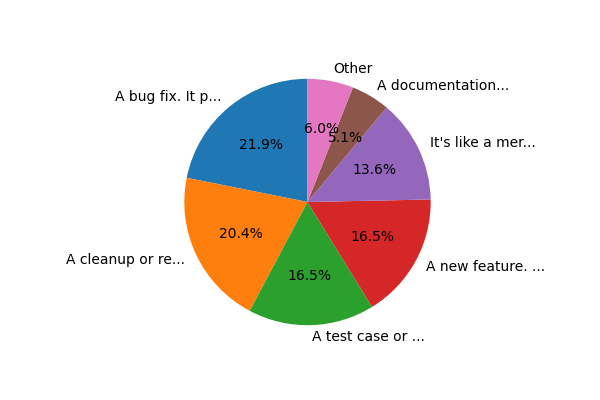
\includegraphics[width=\linewidth]{feature-analysis/commit_pie_chart_commit_classification.png}
    \caption{Commit Classification Distribution}
    \label{fig:commit_pie_chart_commit_classification}
\end{figure}

Most commits are focused on bug fixes and cleanups, reflecting efforts to maintain code quality. Testing infrastructure changes are also significant, showing the emphasis on robustness. New features make up a large portion of the commits, while merge commits are typical in the Linux kernel.

\paragraph{Commit Complexity Distribution}
\begin{figure}[ht]
    \centering
    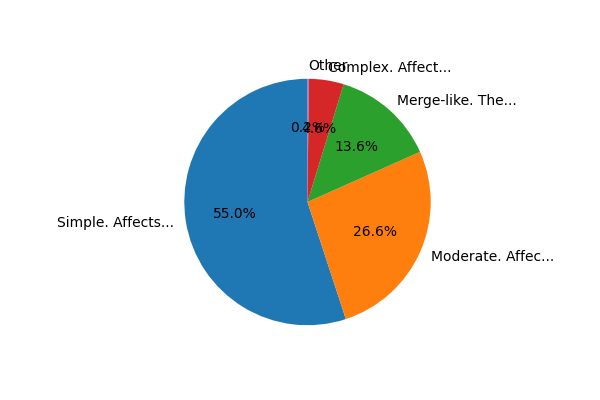
\includegraphics[width=\linewidth]{feature-analysis/commit_pie_chart_commit_complexity.png}
    \caption{Commit Complexity Distribution}\label{fig:commit_pie_chart_commit_complexity}
\end{figure}

The majority of commits are simple, involving small changes, while more complex changes make up a smaller, but notable, portion.
\paragraph{Major Related Implementation Components}
\begin{figure}[ht]
    \centering
    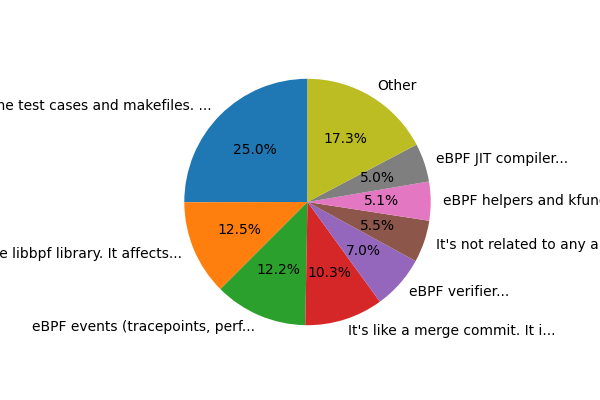
\includegraphics[width=\linewidth]{feature-analysis/commit_pie_chart_major_implementation_component.png}
    \caption{Major Related Implementation Components}\label{fig:commit_pie_chart_major_implementation_component}
\end{figure}

Test cases and build scripts are significantly impacted, highlighting continuous improvements in testing and build processes. \texttt{libbpf} is also a key component in the kernel eBPF toolchain. Additionally, a large amount of development occurs in other kernel subsystems, particularly in relation to eBPF events. The frequency of updates to the eBPF verifier and helpers also indicates ongoing efforts to enhance functionality and ensure program safety. Notably, some commits seems not related to eBPF subsystems.

\paragraph{Logic Components Affected}
\begin{figure}[ht]
    \centering
    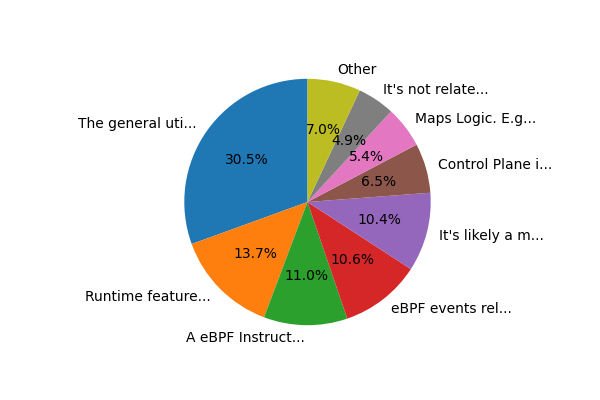
\includegraphics[width=\linewidth]{feature-analysis/commit_pie_chart_major_logic_component.png}
    \caption{Major Related Logic Components}
\end{figure}

General utilities, such as tools and scripts, see the most updates, followed by runtime features like helpers and kernel functions, which are consistently enhanced. eBPF event logic and instruction handling are also frequently updated to ensure robustness and functionality.
 
\paragraph{Use Cases and eBPF Events}
\begin{figure}[ht]
    \centering
    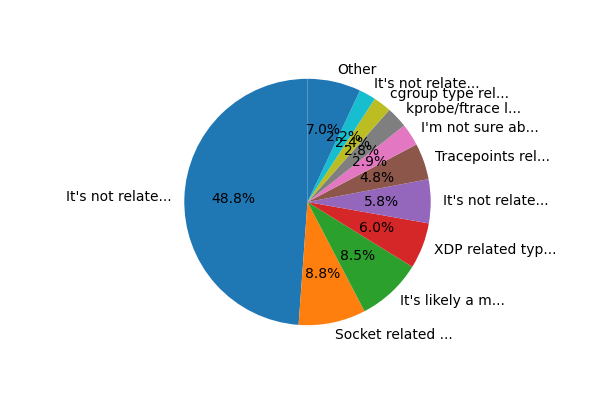
\includegraphics[width=\linewidth]{feature-analysis/commit_pie_chart_usecases_or_submodule_events.png}
    \caption{Related Events and Use Cases}
\end{figure}

While most commits enhance core eBPF infrastructure, including the verifier and runtime components, their development 
Networking-related features, such as socket and XDP programs, receive significant attention, while tracing tools like tracepoints and kprobes show eBPF's important role in system diagnostics and debugging.

\subsection{Correctness of Survey Responses}

To ensure survey responses accurately reflect system features and commits, we validate responses by randomly sampling the data and cross-referencing with expert knowledge and processing logs. Specifically, we addressed two common issues: the handling of merge commits and the identification of commits unrelated to the BPF subsystem.

\subsubsection{Merge Commit Correctness}

For merge commits, we observed a discrepancy between the commit classification perspective and the major implementation component perspective.  To address this, we analyzed the top merge commit messages and determined that some merge commits were categorized based on their predominant effect on a specific component rather than being uniformly labeled as merge commits. By making this clear in the survey questions, we ensured that the survey's classification system accounted for these distinctions and reflected the correct commit impact across perspectives.

\textbf{Example:}
\begin{verbatim}
Top Commit (Classification but not Implementation):
3    Merge branch 'bpf-fix-incorrect-name-check-pass'
25   Merge branch 'vsc73xx-fix-mdio-and-phy' Pawel...
\end{verbatim}

\subsubsection{Non-Related BPF Subsystem Commits}

We noted that commits not directly related to the BPF subsystem were sometimes included due to broad filtering criteria (e.g., \textbf{--grep=bpf}). After reviewing these commits, we confirm some commits mentioned "bpf" but addressed unrelated or peripheral issues.

\textbf{Example:}
\begin{verbatim}
Sample 'Not related to BPF' Commit Messages:
17    bonding: fix xfrm real_dev null pointer...
21    btrfs: fix invalid mapping of extent xarray st...
\end{verbatim}

\subsubsection{Consistency Across Similar Questions}

We checked for consistency in responses by comparing related questions, focusing on the merge commit numbers in commit classifications and complexities, and also unrelated components commit numbers in Implementation and logic components.

\textbf{Example 1: Merge Commits}
\begin{itemize}
    \item \textbf{Commit Classification:} "It's like a merge commit." (1,347 responses)
    \item \textbf{Commit Complexity:} "Merge-like. The commit merges branches." (1,346 responses)
\end{itemize}

\textbf{Example 2: Unrelated Components}
\begin{itemize}
    \item \textbf{Implementation Component:} "Not related to BPF." (606 responses)
    \item \textbf{Logic Component:} "Not related to BPF." (602 responses)
\end{itemize}

The close match shows consistent identification of unrelated components. With a low misclassification rate (under 0.05\%), our data shows high consistency, supporting the reliability of the survey design.

\subsection{Timeline Analysis of Commits}

The timeline analysis of commits offers valuable insights into the evolution of the eBPF subsystem over time. By visualizing the distribution of commit types, complexities, and major components across different periods, trends and patterns in the development of eBPF features become evident.

The data was processed by cleaning it to remove irrelevant commits, smoothing it using a 3-month average to reduce noise and highlight long-term trends, and treating single-component \texttt{Merge} commits as regular commits while removing multi-component \texttt{Merge} commits, such as mainline merges. The time span is from 2017 to the end of 2024, with more than 15000 commits.

\subsubsection{Commit Classification Over Time}
\begin{figure}[ht]
    \centering
    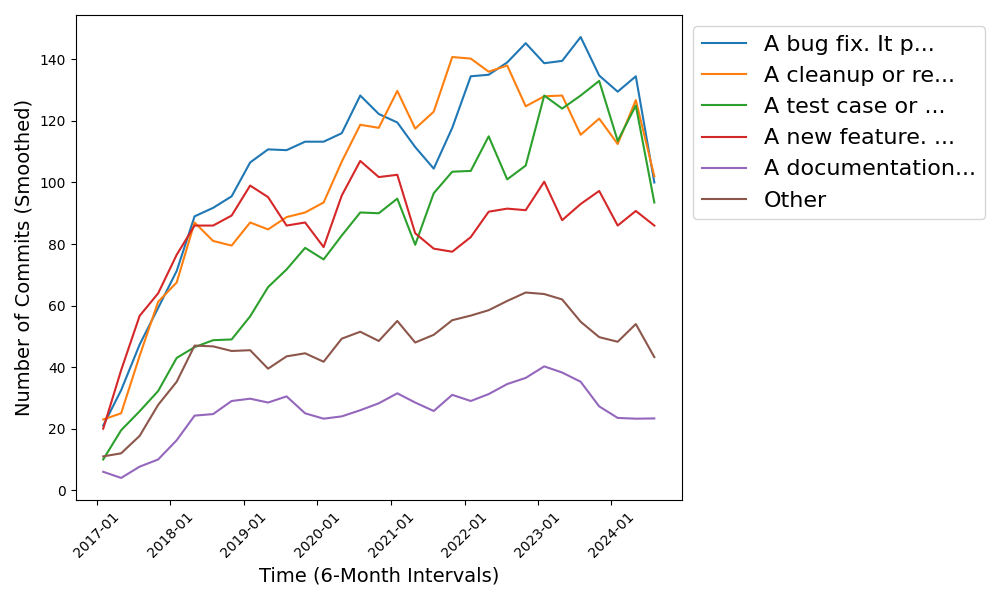
\includegraphics[width=\linewidth]{feature-analysis/timeline_commit_classification_smoothed.png}
    \caption{Commit Classification Over Time}\label{fig:timeline_commit_classification_smoothed}
\end{figure}
\Cref{fig:timeline_commit_classification_smoothed} shows the distribution of different types of code commits over time.

The development started to grow significantly in 2017, but the addition of test cases was limited at first and continued to improve later. New feature development follows a cyclical pattern, with notable spikes around 2020 and 2021. After 2021, the number of cleanups and refactoring increases significantly, while new feature additions decline, indicating a shift in focus towards code maintainability and stability. A decline of cleanup commits after 2023 suggests that while new features continue to be added, the focus has shifted more towards stabilization and optimization.

\subsubsection{Commits Related to Major Implementation Components Over Time}
\begin{figure}[ht]
    \centering
    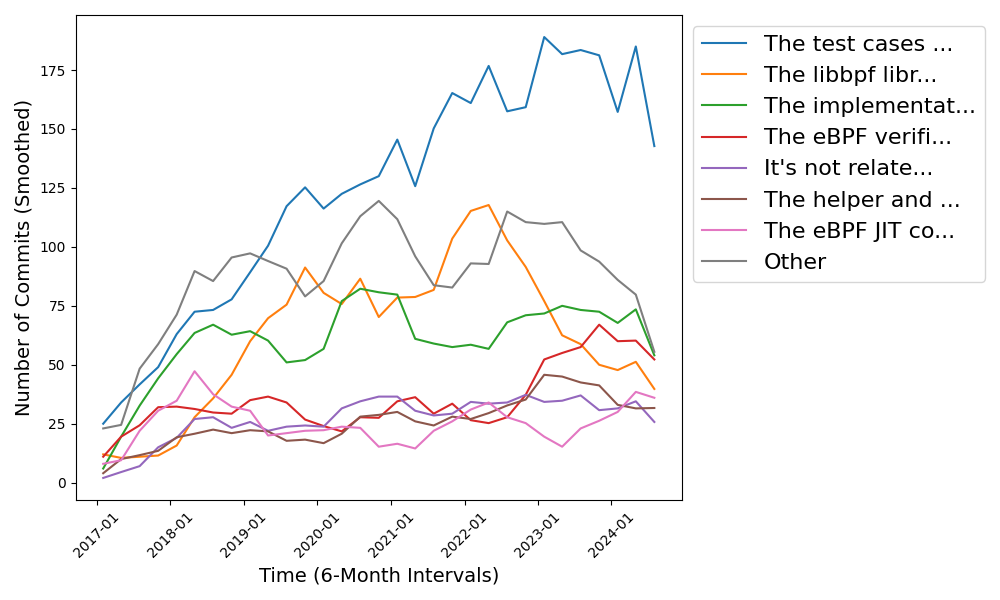
\includegraphics[width=\linewidth]{feature-analysis/timeline_major_related_implementation_component_smoothed.png}
    \caption{Commits Related to Major Implementation Components Over Time}\label{fig:timeline_major_related_implementation_component_smoothed}
\end{figure}

\Cref{fig:timeline_major_related_implementation_component_smoothed} shows the evolution of major implementation components in the Linux BPF subsystem.

Most components see their highest activity between 2017 and 2022, reflecting the rapid development of eBPF features during this time. The libbpf library saw the most dramatic increase, while the JIT compiler was most frequently updated around 2018. The rise in test cases also reflects the growing importance of a robust testing framework being introduced in this field.

After peaking around 2021-2022, several components show a decline or stabilization in activity. This indicates that many eBPF components have entered a phase of optimization and maintenance rather than new feature development, while testing continues to be applied to increase coverage. The verifier shows modest activity throughout the observed period but seems to increase in 2023-2024, which may reflect renewed research efforts in this area.
 
\subsubsection{Commit Related to Major Logic Component Over Time}
\begin{figure}[ht]
    \centering
    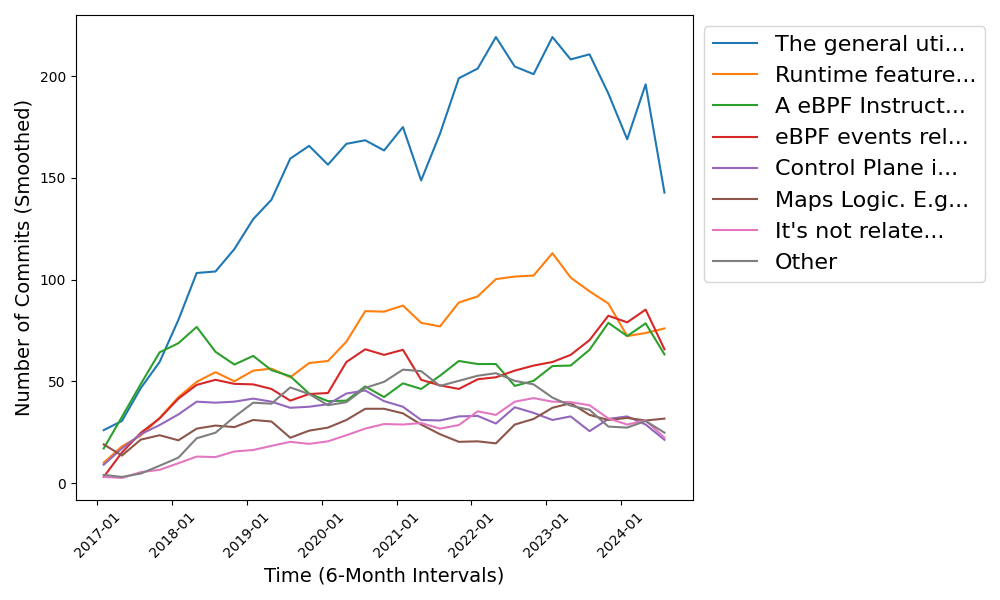
\includegraphics[width=\linewidth]{feature-analysis/timeline_major_related_logic_component_smoothed.png}
    \caption{Commit Related to Major Logic Components Over Time}\label{fig:timeline_major_related_logic_component_smoothed}
\end{figure}
\Cref{fig:timeline_major_related_logic_component_smoothed} depicts the evolution of major logic components in Linux BPF subsystem. 

Figure \ref{fig:timeline_major_related_logic_component_smoothed} shows the number of commits for various logic components or features. Most improvements are around The general utilities" component, which peaks around 2022-2023 before decreasing. Other components like "Runtime features, helpers and kfuncs" and "eBPF Instruction Logic" show more gradual increases over time, while components such as "Control Plane interface" and "Maps Logic" maintain relatively steady levels of activity throughout the period.

\subsubsection{Use Cases or Events Over Time}

\begin{figure}[ht]
    \centering
    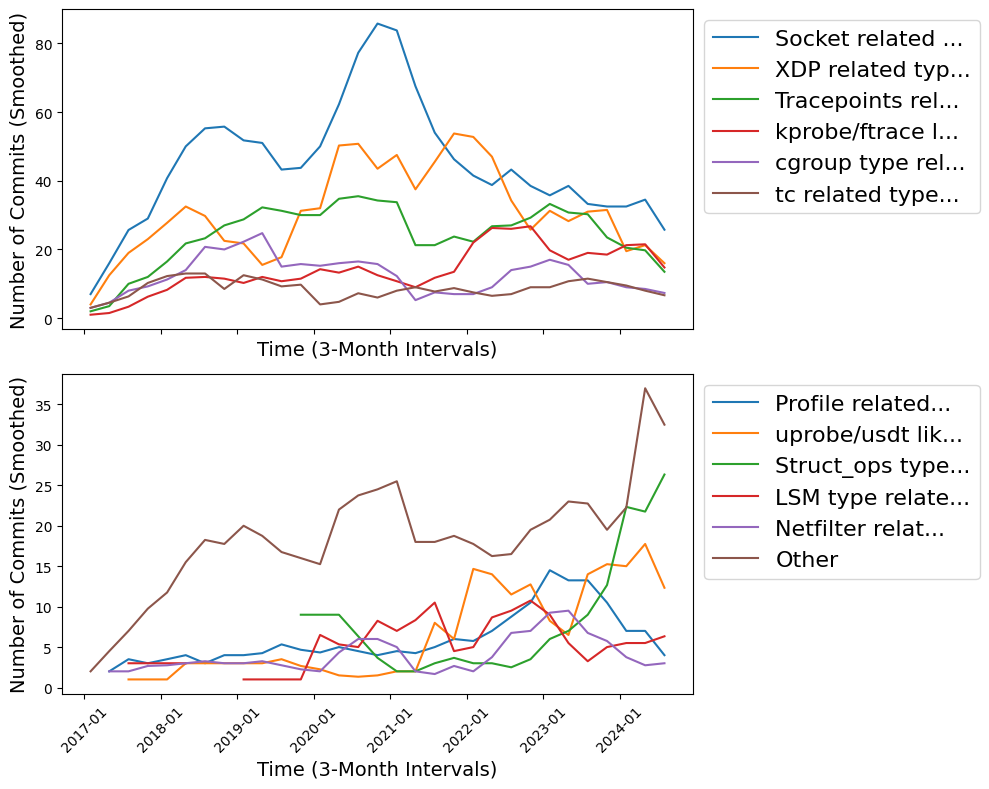
\includegraphics[width=\linewidth]{feature-analysis/timeline_usecases_or_submodule_events_smoothed.png}
    \caption{Use Cases or Events Over Time }\label{fig:timeline_usecases_or_submodule_events_smoothed}
\end{figure}

\Cref{fig:timeline_usecases_or_submodule_events_smoothed} reveals significant fluctuations in event types over the years.

The most notable are the network-related events, such as socket and XDP programs. There was a surge in both socket- and XDP-related activities from 2020 to 2022, after which they entered a stabilization phase following the initial burst of feature additions and optimizations. The tracepoints-related line shows a steady increase with periodic fluctuations, peaking around 2021 before decreasing. The kprobe/ftrace-related events remain mostly stable, with a slight increase in 2022. uprobe-related events show moderate activity over several years, with a slight peak in 2022 and again in 2024. Struct\_ops, an emerging feature introduced in 2020, shows a significant increase in activity between 2023 and 2024. Other events such as LSM for security are still minor.

\subsection{Deeper Insights Analysis}

This section delves into the survey responses to uncover patterns, trends, and areas for improvement within the eBPF subsystem.
\subsubsection{Which Kernel Components and Files Have the Most Frequent Bugs?}

\begin{figure}[ht]
    \centering
    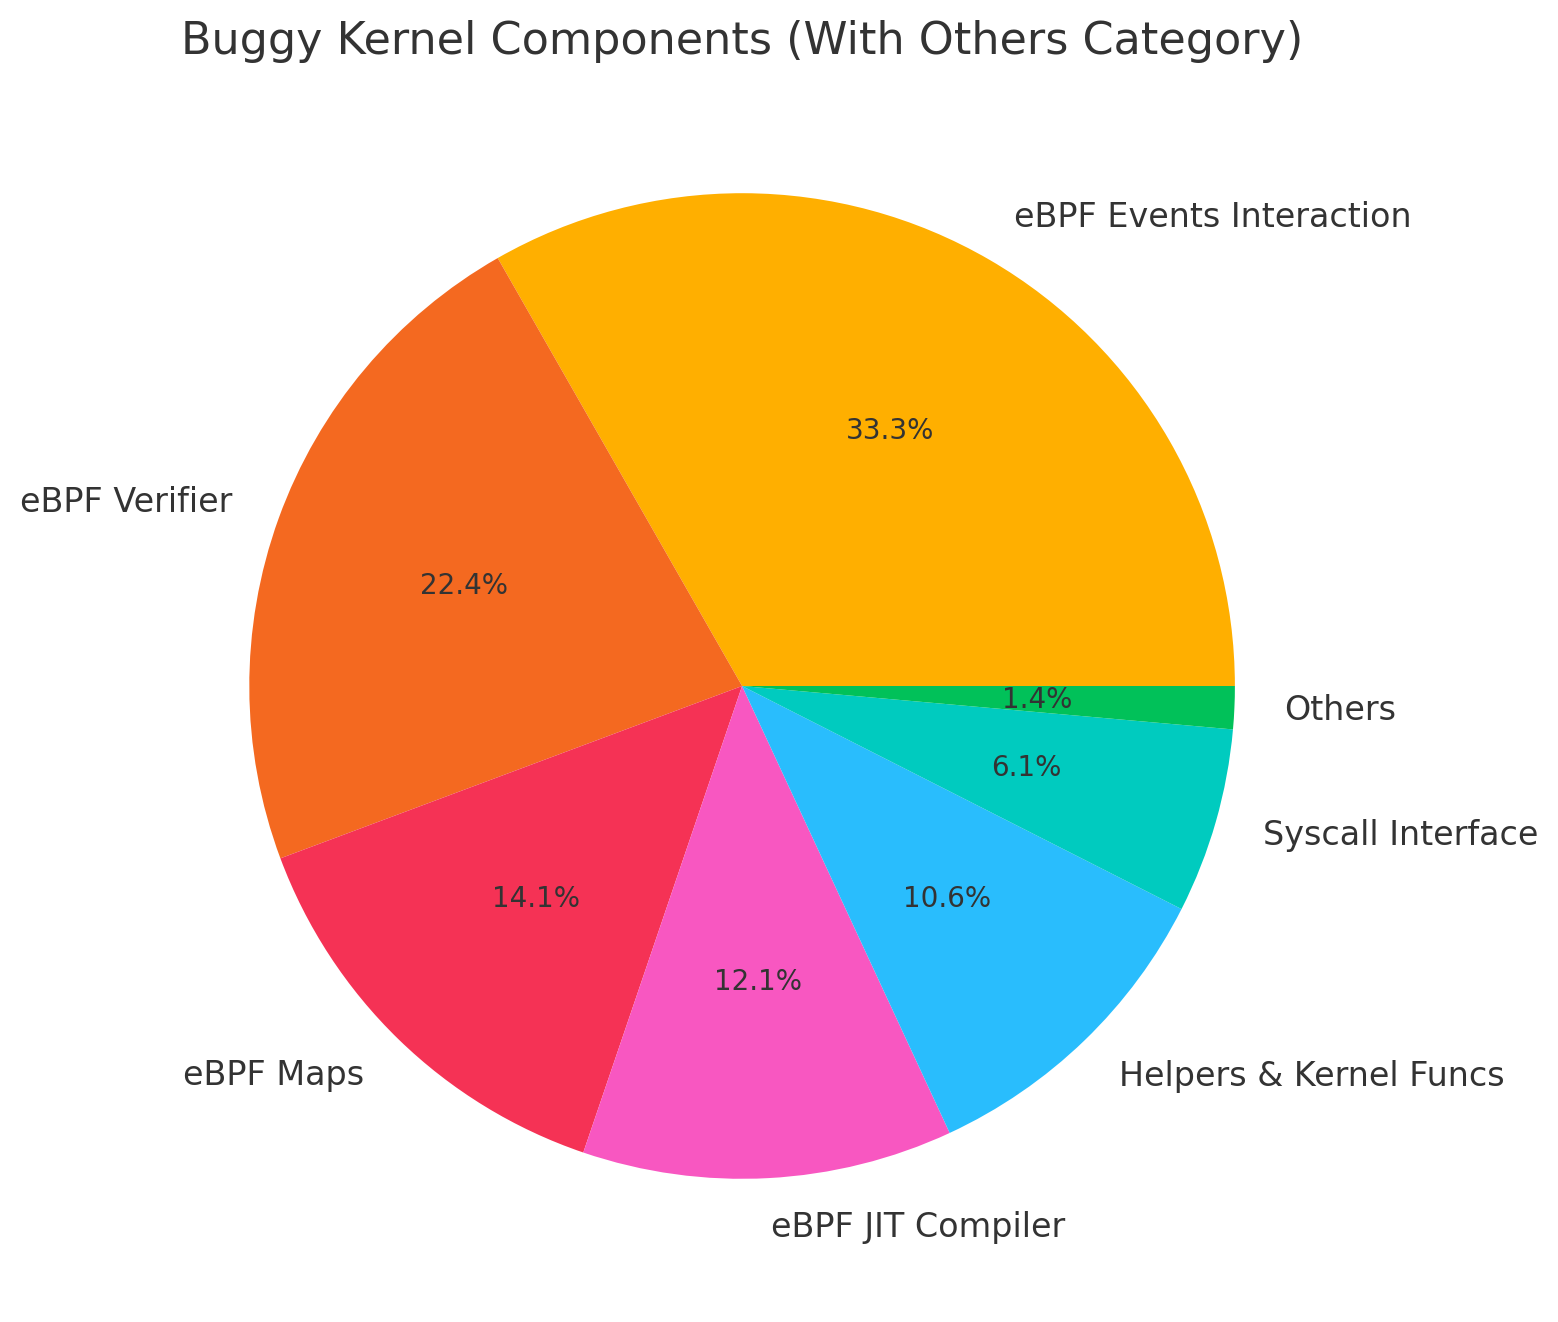
\includegraphics[width=\linewidth]{feature-analysis/commit_pie_buggy_kernel_componenet.png}
    \caption{Verifier Instruction Features vs. General Verifier Bugs Over Time}
    \label{fig:buggy_kernel_component}
\end{figure}

\Cref{fig:buggy_kernel_component} illustrates the kernel implementation components with a large number of bugs. While previous analyses and tools have primarily focused on improving the stability of the verifier and JIT compiler, these areas account for only about 35\% of the bugs. The largest amount of bugs originate from eBPF event-related code, which involves the interaction of eBPF with other kernel subsystems. Additionally, helpers and maps also have a significant number of bugs. Due to the complexity of the control plane, the syscall interface of eBPF is also prone to bugs.

By examining the specific files, we can also observe that bugs frequently occur in the verifier, syscall, core, and network filter components. The kernel needs better coverage and more attention on these files.

\textbf{Top 5 Buggy Files:}
\begin{verbatim}
 kernel/bpf/verifier.c             425
 net/core/filter.c                 140
 kernel/bpf/syscall.c              111
 include/linux/bpf.h                87
 kernel/bpf/core.c                  83
\end{verbatim}


\subsubsection{What is the Relationship Between Instruction-Related Changes in the Verifier and All Verifier Bugs?}

\begin{figure}[ht]
    \centering
    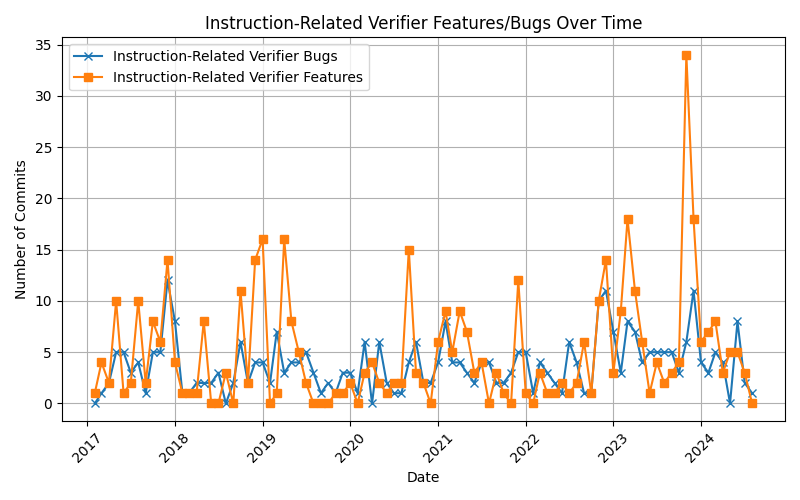
\includegraphics[width=\linewidth]{feature-analysis/instruction_verifier_features_bugs_over_time.png}
    \caption{Verifier Bugs or Features Related to eBPF Instruction Over Time}
    \label{fig:instruction_verifier_features_bugs_over_time}
\end{figure}

\Cref{fig:instruction_verifier_features_bugs_over_time} shows that changes related to eBPF instructions in the verifier are closely related to the number of verifier bugs. This insight highlights the importance of focusing on instruction-related aspects during verifier development and debugging to enhance overall system stability.

\subsubsection{The Evolution and Status of libbpf}

We also examined the lifecycle of specific components, such as \texttt{libbpf}.

Based on \Cref{fig:libbpf_commit_classification}, the development of libbpf began to grow significantly in 2017. New feature development follows a cyclical pattern, with notable spikes around 2020 and 2022. After 2022, the number of cleanups and refactorings increased significantly, indicating a shift in focus towards code maintainability and stability. However, the decline in cleanup commits after 2023 suggests that while new features continue to be added, the focus has shifted more towards stabilization and optimization.

Historical milestones verify this trend. For instance, libbpf version 1.0 was released in August 2022 \cite{libbpf1}, and the major feature "Compile Once, Run Everywhere" (CO-RE) was introduced around 2020 \cite{core}, both aligning with the peaks and shifts observed in the commit history.


\begin{figure}[ht]
    \centering
    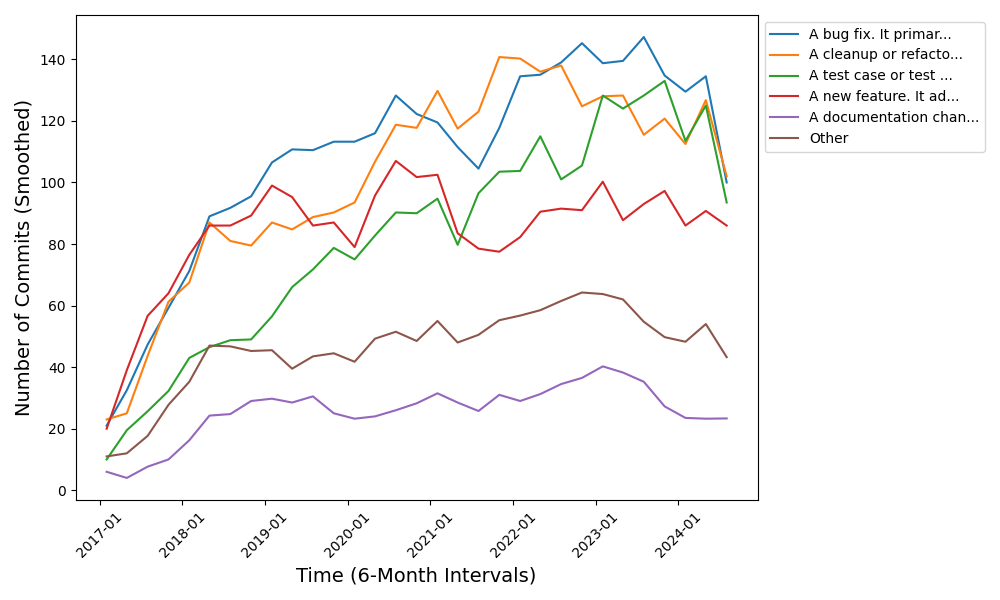
\includegraphics[width=\linewidth]{feature-analysis/timeline_libbpf_commit_classification_smoothed.png}
    \caption{Evolution of \texttt{libbpf} Over Time}
    \label{fig:libbpf_commit_classification}
\end{figure}

\subsection{Expert Confirmation} 

We discussed the results with more than five eBPF experts who have submitted kernel patches or given conference talks. They confirmed that the results are likely correct based on their understanding. We also shared the report with kernel maintainers and the BPF kernel mailing list, which is under discussion. Additionally, we plan to provide experts with a sample of survey responses and ask them to rate the accuracy of each response on a defined scale. Based on their feedback, we will refine the survey to improve its correctness and relevance.

\subsection{Clarity and Ambiguity in Responses}

Based on the insights gathered from the survey responses, the survey results are likely clear and  actionable. We plan to invite more experts to review a sample of the responses to identify any vague or unclear answers. Afterward, we will revise any survey questions prone to misinterpretation or ambiguity to improve clarity and precision.

\subsection{Alignment with Real-World Changes}

By compare survey responses with real-world feature changes discussed before, we confirm that the survey likely captures the correct historical context. We plan to cross-reference survey results with commit histories, mailing list discussions, and kernel release notes to further verify alignment with real-world changes.


\subsection{Coverage of Survey Questions}

We plan to review the survey’s coverage to identify potential gaps, ensuring that important aspects such as security, performance, and dependencies are addressed.

% \begin{figure}
%     \centering
%     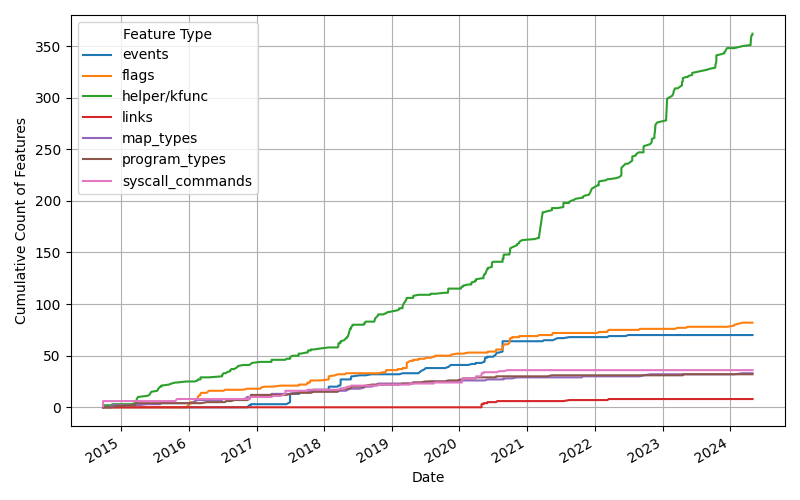
\includegraphics[width=0.5\textwidth]{feature-analysis/cumulative_bpf_features_timeline.png}
%     \caption{Cumulative bpf features timeline}
%     \label{fig:feature}
% \end{figure}

% \begin{figure}
%     \centering
%     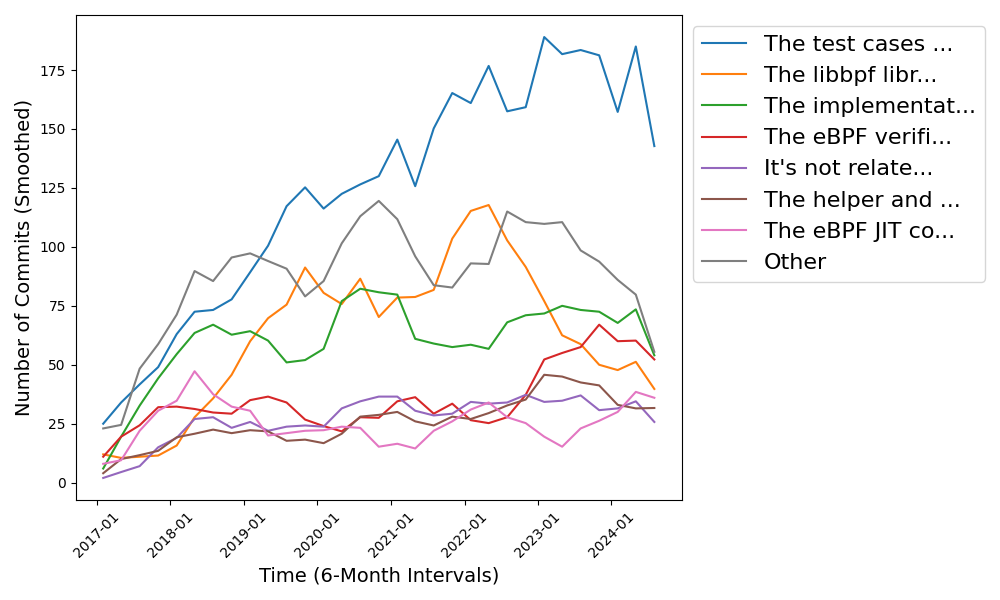
\includegraphics[width=0.5\textwidth]{feature-analysis/timeline_major_related_implementation_component_smoothed.png}
%     \caption{Timeline major related implementation component smoothed}
%     \label{fig:smoothed}
% \end{figure}